\documentclass{article}
\usepackage[a4paper,top=0.75in, bottom=0.75in, left=1in, right=1in,footskip=0.2in]{geometry}
%\usepackage{fullpage}
\usepackage{listings}
\usepackage{gensymb}
\usepackage{hyperref}
\hypersetup{
	 colorlinks   = true,
     citecolor    = black,
     linkcolor    = black,
     urlcolor     = black
}
\usepackage{graphicx}
\usepackage{algorithm}
\usepackage{algpseudocode}
\usepackage{amsmath}
\usepackage{amssymb}
\usepackage{tikz}
\usepackage{caption}
\usepackage{subcaption}
\usepackage{float}
\usetikzlibrary{arrows,matrix,positioning}
\setcounter{tocdepth}{3}
\begin{document}
\title{DIP Homework 4}
\author{Qiuyi Zhang 12330402 \\ \href{mailto:joyeec9h3@gmail.com}{joyeec9h3@gmail.com}} 
\date{\today}
\maketitle
\tableofcontents
\section{Exercises}

\subsection{Color Spaces}

\textbf{Answer:} 

\begin{enumerate}
\item Advantages of HSI color space:
\begin{enumerate}
\item xxx
\item xxx
\end{enumerate}

\item Adding $120\degree$ to the Hue components
\end{enumerate}

\subsection{Color Composition}

\textbf{Answer:}

General expression


% -------------------- Programming Tasks ------------------------
\section{Programming Tasks}
% -------------------- Fourier Transform ------------------------
\subsection{Image Filtering}
% -------------------- Results ------------------------

\begin{figure}[H]
	\centering
	% pt = px * 72 / DPI
	
\includegraphics[width=192pt]{../img/task_1.png}
	\caption{The original image}
\end{figure}

\subsubsection{Arithmetic mean filter}

The images filtered with $3 \times 3$ and $9 \times 9$ arithmetic mean filters are shown in Figure~\ref{fig:baram33} and~\ref{fig:baram99}

\begin{figure}[H]
	\captionsetup{justification=centering,margin=1cm}
	\begin{minipage}[b]{0.48\linewidth}
		\centering
		% pt = px * 72 / DPI
		
\includegraphics[width=192pt]{../result/task1/arithmetic-mean-3-3.png}
		\caption{Filtered with $3 \times 3$ arithmetic mean filter}
		\label{fig:baram33}
	\end{minipage}
	\begin{minipage}[b]{0.48\linewidth}
		\centering
		% pt = px * 72 / DPI
		
\includegraphics[width=192pt]{../result/task1/arithmetic-mean-9-9.png}
		\caption{Filtered with $9 \times 9$ arithmetic mean filter}
		\label{fig:baram99}
	\end{minipage}
\end{figure}


\subsubsection{Harmonic mean filter}

The images filtered with $3 \times 3$ and $9 \times 9$ harmonic mean filters are shown in Figure~\ref{fig:barhm33} and~\ref{fig:barhm99}
\begin{figure}[H]
	\captionsetup{justification=centering,margin=1cm}
	\begin{minipage}[b]{0.48\linewidth}
		\centering
		% pt = px * 72 / DPI
		
\includegraphics[width=192pt]{../result/task1/harmonic-mean-3-3.png}
		\caption{Filtered with $3 \times 3$ harmonic mean filter}
		\label{fig:barhm33}
	\end{minipage}
	\begin{minipage}[b]{0.48\linewidth}
		\centering
		% pt = px * 72 / DPI
		
\includegraphics[width=192pt]{../result/task1/harmonic-mean-9-9.png}
		\caption{Filtered with $9 \times 9$ harmonic mean filter}
		\label{fig:barhm99}
	\end{minipage}
\end{figure}

\subsubsection{Contraharmonic mean filter}

The images filtered with $3 \times 3$ and $9 \times 9$ contraharmonic mean filters are shown in Figure~\ref{fig:barchm33} and~\ref{fig:barchm99}

\begin{figure}[H]
	\captionsetup{justification=centering,margin=1cm}
	\begin{minipage}[b]{0.48\linewidth}
		\centering
		% pt = px * 72 / DPI
		
\includegraphics[width=192pt]{../result/task1/contraharmonic-mean-3-3.png}
		\caption{Filtered with $3 \times 3$ contraharmonic mean filter}
		\label{fig:barchm33}
	\end{minipage}
	\begin{minipage}[b]{0.48\linewidth}
		\centering
		% pt = px * 72 / DPI
		
\includegraphics[width=192pt]{../result/task1/contraharmonic-mean-9-9.png}
		\caption{Filtered with $9 \times 9$ contraharmonic mean filter}
		\label{fig:barchm99}
	\end{minipage}
\end{figure}

% End results and descirptions


\subsection{Image Denoising}

\subsubsection{Statistical filters}

\paragraph{Algorithm}
Discuss how you implement this operation in less than 1 page.

\begin{figure}[]
	\centering
	% pt = px * 72 / DPI
	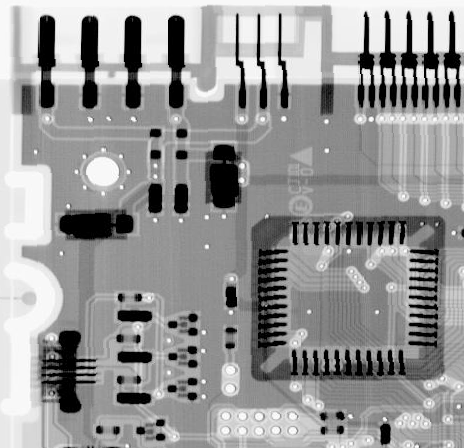
\includegraphics[width=336pt]{../img/task_2.png}
	\caption{The original image}
\end{figure}

\subsubsection{Gaussian noise and denoising}

\paragraph{Results}
\begin{figure}[H]
	\centering
	% pt = px * 72 / DPI
	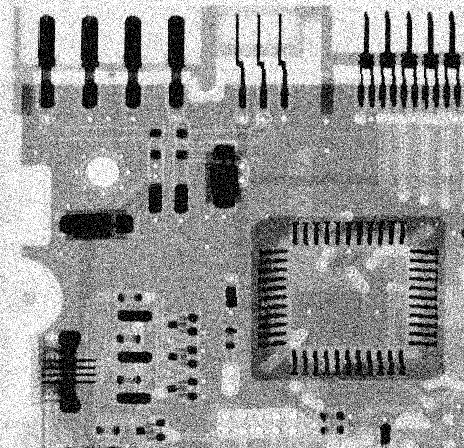
\includegraphics[width=336pt]{../result/task2/gauss/gauss-0-40.png}
	\caption{Image with gaussian noise($\mu = 0, \sigma = 40$)}
	\label{fig:gauss}
\end{figure}

\begin{figure}[H]
	\centering
	% pt = px * 72 / DPI
	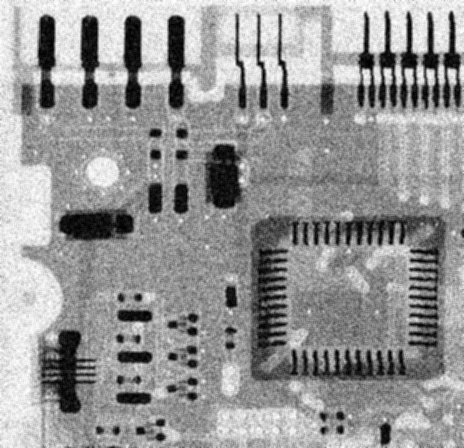
\includegraphics[width=336pt]{../result/task2/gauss/gauss-arithmetic.png}
	\caption{Gaussian noise filtered with $3 \times 3$ arithmetic mean filter}
	\label{fig:gaussam}
\end{figure}

\begin{figure}[H]
	\centering
	% pt = px * 72 / DPI
	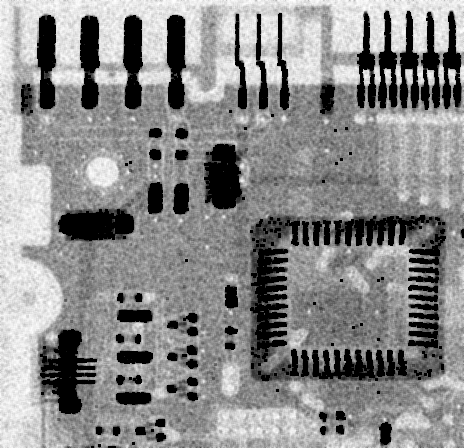
\includegraphics[width=336pt]{../result/task2/gauss/gauss-geometric.png}
	\caption{Gaussian noise filtered with $3 \times 3$ geometric mean filter}
	\label{fig:gaussgm}
\end{figure}

\begin{figure}[H]
	\centering
	% pt = px * 72 / DPI
	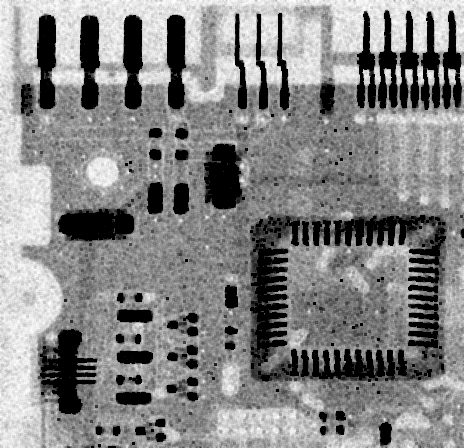
\includegraphics[width=336pt]{../result/task2/gauss/gauss-harmonic.png}
	\caption{Gaussian noise filtered with $3 \times 3$ harmonic mean filter}
	\label{fig:gausshm}
\end{figure}

\begin{figure}[H]
	\centering
	% pt = px * 72 / DPI
	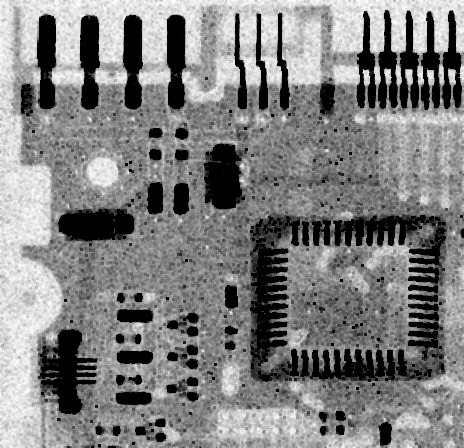
\includegraphics[width=336pt]{../result/task2/gauss/gauss-contraharmonic.png}
	\caption{Gaussian noise filtered with $3 \times 3$ contraharmonic mean filter($Q = -1.5$)}
	\label{fig:gausschm}
\end{figure}

\begin{figure}[H]
	\centering
	% pt = px * 72 / DPI
	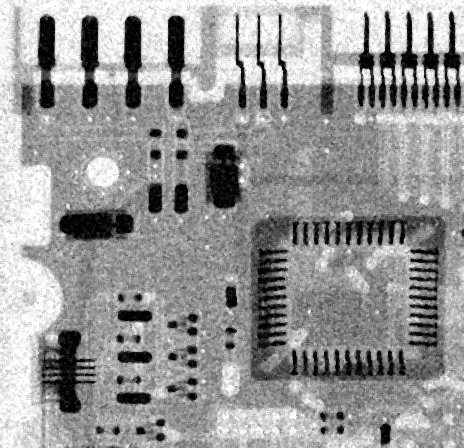
\includegraphics[width=336pt]{../result/task2/gauss/gauss-median.png}
	\caption{Gaussian noise filtered with $3 \times 3$ median filter}
	\label{fig:gaussm}
\end{figure}


\paragraph{Discussion}
Compare these results, and discuss which one looks better / worse, and why, within 1 page

\subsubsection[H]{Salt noise and denoising}

\paragraph{Results}

\begin{figure}[H]
	\centering
	% pt = px * 72 / DPI
	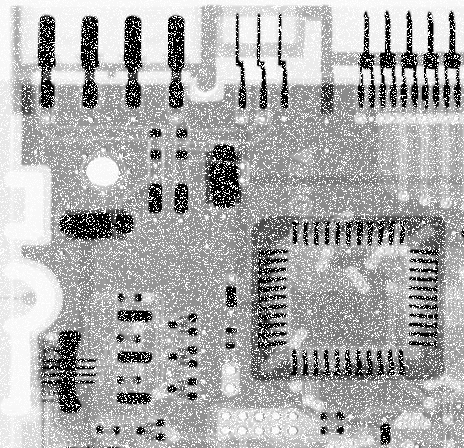
\includegraphics[width=336pt]{../result/task2/salt/salt-20.png}
	\caption{Image with salt noise($p=0.2$)}
	\label{fig:salt}
\end{figure}

\begin{figure}[H]
	\centering
	% pt = px * 72 / DPI
	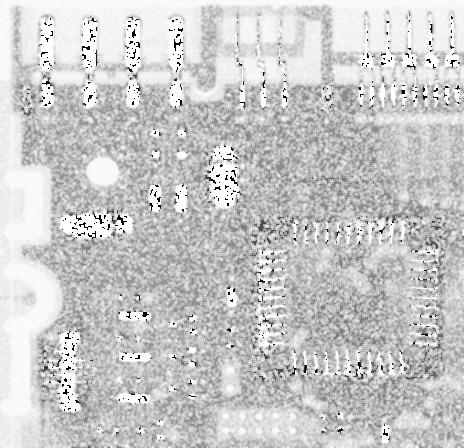
\includegraphics[width=336pt]{../result/task2/salt/salt-contraharmonic-1-5.png}
	\caption{Salt noise filtered with $3 \times 3$ contraharmonic mean filter($Q = 1.5$)}
	\label{fig:saltchmpos}
\end{figure}

\begin{figure}[H]
	\centering
	% pt = px * 72 / DPI
	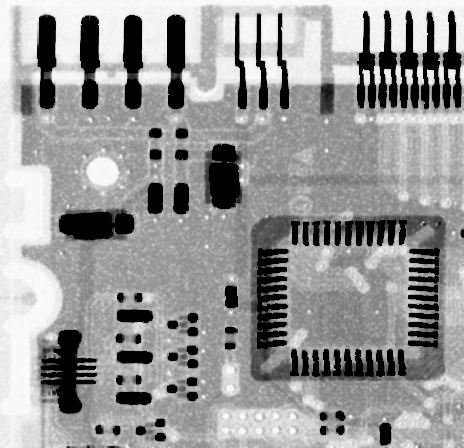
\includegraphics[width=336pt]{../result/task2/salt/salt-contraharmonic--1-5.png}
	\caption{Salt noise filtered with $3 \times 3$ contraharmonic mean filter($Q = -1.5$)}
	\label{fig:saltchmneg}
\end{figure}

\paragraph{Discussion}
Discuss why setting a wrong value for Q would lead to terrible results within 1 page.

\subsubsection{Salt-and-pepper noise and denoising}
\paragraph{Results}


\begin{figure}[H]
	\centering
	% pt = px * 72 / DPI
	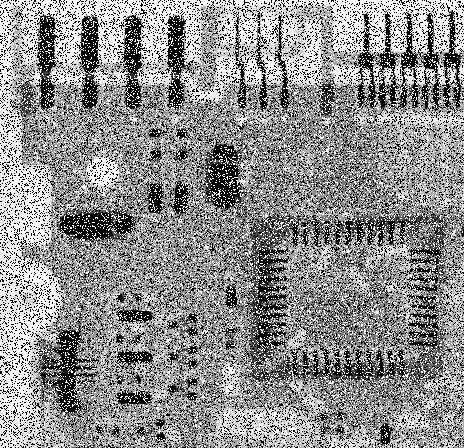
\includegraphics[width=336pt]{../result/task2/sap/sap-20-20.png}
	\caption{Image with salt noise($p=0.2$) and pepper noise($p=0.2$)}
	\label{fig:sap}
\end{figure}

\begin{figure}[H]
	\centering
	% pt = px * 72 / DPI
	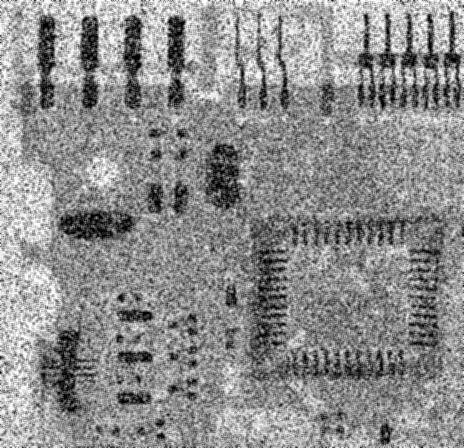
\includegraphics[width=336pt]{../result/task2/sap/sap-arithmetic.png}
	\caption{Salt-and-pepper noise filtered with $3 \times 3$ arithmetic mean filter}
	\label{fig:sapam}
\end{figure}

\begin{figure}[H]
	\centering
	% pt = px * 72 / DPI
	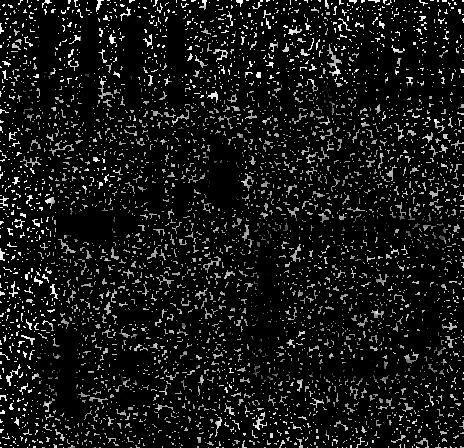
\includegraphics[width=336pt]{../result/task2/sap/sap-harmonic.png}
	\caption{Salt-and-pepper filtered with $3 \times 3$ harmonic mean filter}
	\label{fig:saphm}
\end{figure}


\begin{figure}[H]
	\centering
	% pt = px * 72 / DPI
	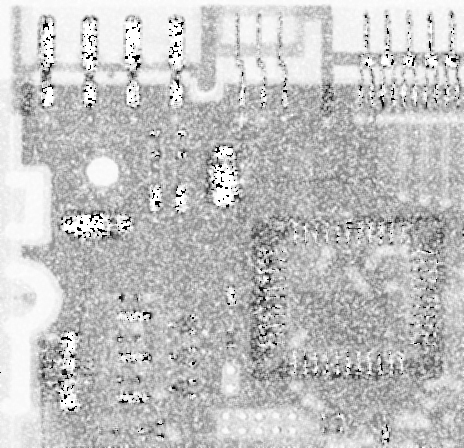
\includegraphics[width=336pt]{../result/task2/sap/sap-contraharmonic.png}
	\caption{Salt-and-pepper noise filtered with $3 \times 3$ contraharmonic mean filter($Q=0.5$)}
	\label{fig:sapchm}
\end{figure}

\begin{figure}[H]
	\centering
	% pt = px * 72 / DPI
	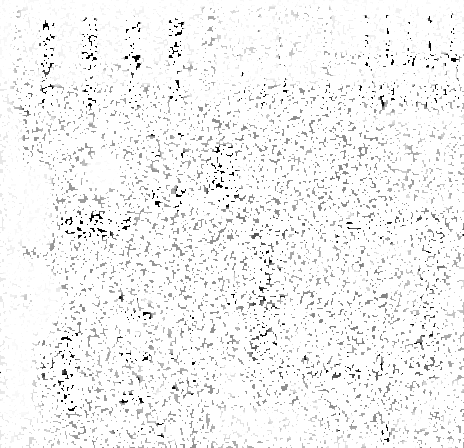
\includegraphics[width=336pt]{../result/task2/sap/sap-max.png}
	\caption{Salt-and-pepper noise filtered with $3 \times 3$ max filter}
	\label{fig:sapmax}
\end{figure}

\begin{figure}[H]
	\centering
	% pt = px * 72 / DPI
	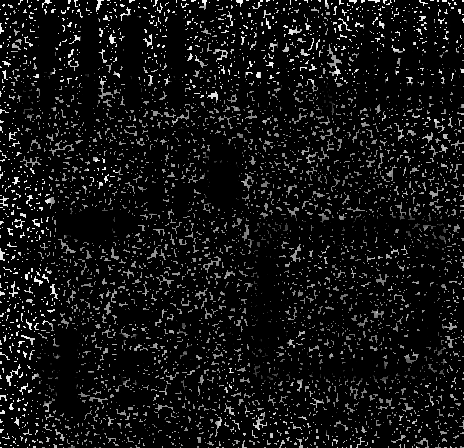
\includegraphics[width=336pt]{../result/task2/sap/sap-min.png}
	\caption{Salt-and-pepper noise filtered with $3 \times 3$ min filter}
	\label{fig:sapmin}
\end{figure}

\begin{figure}[H]
	\centering
	% pt = px * 72 / DPI
	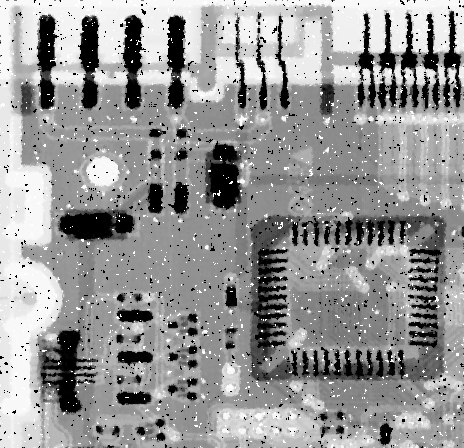
\includegraphics[width=336pt]{../result/task2/sap/sap-median.png}
	\caption{Salt-and-pepper noise filtered with $3 \times 3$ median filter}
	\label{fig:sapmedian}
\end{figure}

\paragraph{Discussion}
Compare these results, and discuss which one looks better / worse, and why, within 1 page

\subsection{Histogram Equalization on Color Images}

\subsubsection{Results}

\begin{figure}[H]
	\centering
	% pt = px * 72 / DPI
	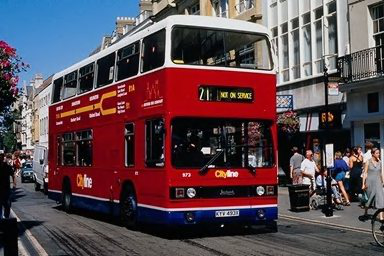
\includegraphics[width=288pt]{../img/02.png}
	\caption{The original image}
\end{figure}

\begin{figure}[H]
	\centering
	% pt = px * 72 / DPI
	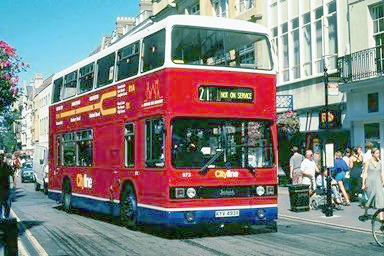
\includegraphics[width=288pt]{../result/hist/hist-seperate.png}
	\caption{Image rebuilt with three channels equalized with different histograms}
\end{figure}

\begin{figure}[h]
	\centering
	% pt = px * 72 / DPI
	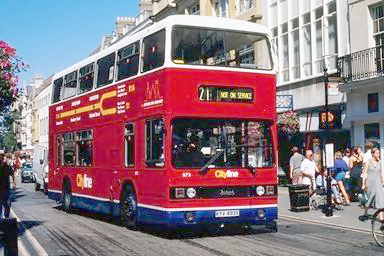
\includegraphics[width=288pt]{../result/hist/hist-together.png}
	\caption{Image rebuilt with three channels equalized with the same average histogram}
\end{figure}


\end{document}